\chapter{MCTDH Theorie}

\section{MCTDH}
Die Effizienz des MCTDH-Verfahrens resultiert aus der Doppellayerstruktur der verwendeten Wellenfunktion. In anderen Wellenpaktendynamikverfahren, 
wie der Standardmethode \cite{MCTDHreview3} wird die Wellenfunktion direkt in einer zeitunabh"angigen Basis oder einem zeitunabh"angigen Gitter entwickelt. 
Anstelle die Wellenfunktion in einer zeitunab"angigen Basis zu entwickeln,
wird im MCTDH-Verfahren das korrelierte mehrdimensionale Wellenpaket als ein Satz von zeitabh"angigen Basisfunktionen dargestellt.
Diese zeitabh"angigen Basisfunktionen werden Einteilchenfunktionen (SPF) genannt. Die SPFs werden in der primitiven zeitunabh"angigen Basis oder Gitter dargestellt.
Das MCTDH-Verfahren kann als eine Zweilayerdarstellung angesehen werden:
So bilden die Entwicklungskoeffizienten, die genutzt werden, um die korrelierte Wellenfunktion in dem Satz der SPF-Basis darzustellen, den oberen Layer der Darstellung.
Die zeitabh"angigen Entwicklungskoeffizienten, die die zeitabh"angigen SPFs in der primitiven zeitunabh"angigen Basis oder Gitter darstellt, bilden den unteren Layer.
Die Bewegungsgleichungen, durch die gleichzeitig die optimale Entwicklungskoeffizienten f"ur beide Layer bestimmt werden, ergeben sich aus dem Dirac-Frenkel Variationsprinzip.
   \\ Dennoch ist auch das MCTDH durch die Anzahl der korrelierten Koordinaten limitiert. 
Die Effizienz des MCTDH-Verfahrens resultiert aus der Gr"o"se der SPF-Basis, die verglichen mit der primitiven Basis signifikant kleiner gew"ahlt werden.
Allerdings skaliert der numerische Aufwand des MCTDH-Verfahrens exponentielle mit der Anzahl der korrelierten Koordinaten.
Um Korrelationseffekte beschreiben zu k"onnen, sind mindestens zwei SPFs in jeder dieser Koordinaten notwendig.
Die Anzahl der Konfigurationen, die in der MCTDH-Wellenfunktion enthalten ist, betr"agt bei $ f $ korrelierten Koordinaten $ 2^f $ Konfigurationen.
Aufgrund dieser Limitierung konnten mit dem MCTDH-Verfahren Systeme mit maximal 12 - 14 korrelierten Koordinaten  berechnet werden.\cite{HM1, HM2, HM4, WWM, WWM2, HM5,
 WMC, BWHHM}
  \\ Das Moden-Kombinationsverfahren wurde von Meyer und seinen Mitarbeitern eingef"uhrt \cite{EMC, WMC2}, das die Anzahl der Konfigurationen reduziert.
Im Moden\-Kombinations\-verfah\-ren werden die ,,logische`` Koordinaten, die in der MCTDH-Darstellung verwendet werden, von physikalischen Koordinaten unterschieden. 
Es werden verschiedene physikalische Koordinaten werden zu einzelnen logischen Koordinaten kombiniert.
Analog zur Theorie der Elektronenstruktur werden diese mehrdimensionalen logischen Koordinaten Partikel genannt. 
Folglich sind die MCTDH Rechnung statt der korrelierten Koordinaten durch die Partikel limitiert. 
So konnten Systeme mit 15 - 24 korrelierten Freiheitsgraden \cite{H5O2+MCTDH2, H5O2+MCTDH3, RWMC, CWMC}
und System-Bad-Modelle \cite{W, WTM, NM2} durch das MCTDH\-Moden\-Kombinations\-verfahren behandelt werden.
Zwar konnte durch dieses Verfahren Grenz zu h"oherer Dimensionalit"at verwschoben werden,
 dennoch bleibt die grundlegende Einschr"ankung: Der numerische Aufwand skaliert mindestens $2^p$, wobei $ p $ die Anzahl der logischen Koordinaten bzw.
 Partikel widergibt. Die Anzahl an physikalischen Koordinaten, die zu logische Koordinaten zusammengefasst werden k"onnen, ist begrenzt, da die SPFs
 nun mehrdimensionale Wellenfunktionen darstellen. F"ur molekulare Systeme stellte sich heraus, dass die Kombination von mehr als drei bis vier Koordinaten in einem Partikel
ineffizient ist.
 \\Die Begrenzung durch die Anzahl der korrelierten Koordinaten bzw. Partikel konnte durch das multilayer (ml)-MCTDH-Verfahren \cite{WT3} "uberwunden werden.
Die SPFs des MCTDH-Verfahrens k"onnen ebenfalls als MCTDH-Wellenfunktion dargestellt werden.
Im daraus resultierende Zweilayer-MCTDH wird eine Dreilayerdarstellung der Wellenfunktion genutzt.:
Der obersten Layer wird durch die zeitabh"angigen Entwicklungskoeffizienten gebildet. Die Wellenfunktion wird in der ersten Layer-SPF-Basis dargestellt, d.h.
SPFs des einfachen MCTDHs. Der mittlere Layer wird durch die zeitabh"angigen Entwicklungskoeffizienten gebilde, die SPFs des ersten Layers in der
SPF-Basis des zweiten Layers darstellen. Die zweite Layer-SPF-Basis ist der zus"atzliche Layer, der im ml-MCTDH-Verfahren dazugekommen ist.
Schlie"slich wird der unterste Layer durch die zeitabh"angigen Entwicklungskoeffizienten gebildet, die die zweite Layer-SPF-Basis in der 
primitiven zeitunabh"angigen Basis oder Gitter dargestellt.
Durch eine rekursive Anwendung der MCTDH-Verfahrens k"onnen weitere Layer hinzugef"ugt werden.
Mit dem ml-MCTDH-Verfahren sind quantumdynamische Rechnungen von System-Bad Modellen mit bis zu 1000 korrelierten Koordinaten m"oglich,
in denen Elektronentransferprozesse \cite{WT3, WST} untersucht wurden.
 \\Um die MCTDH-Wellenfunktion propagieren zu k"onnen, m"ussen die Matrixelemente des Hamiltonoperators effizient berechnet werden.
So lange der Hamiltonoperator der Summe von Produkten von Einteilchenoperatoren \cite{MMC1} entspricht, stellt die Berechnung der Matrixelemente kein Problem dar.
Im Gegensatz zu vielen Modelhamiltonoperatoren k"onnen \textit{ab initio} Potentialenergiefl"achen aber nicht in dieser Form dargestellt werden.
Durch die Verwendung einer spezifischen zeitabh"angigen Quadratur, die die Matrixelemente allgemeiner Potentiale effizient auswertet, k"onnen
auch Matrixelemente solcher \textit{ab initio} Potentialenergiefl"achen effizient berechnet werden.
Diese Vorgehensweise wird correlation discrete variable representation (CDVR) \cite{M3, vHM2} genannt.
 \\Das urspr"ungliche Vorgehen f"ur das CDVR \cite{M3} beruht auf ein zeitabh"angiges DVR-Gitter, das einer SPF-Basis entspricht.
Somit kann das Standard-CDVR weder f"ur modenkombinierte MCTDH-Rechnungen noch f"ur Berechnungen mit dem ML-MCTDH-Ansatz verwendet werden.
 \\Allerdings konnte ein CDVR , das ohne ein direktes Produktgitter auskommt, in modenkombinierte MCTDH-Rechnungen verwendet werden. \cite{vHM3}
 Der numerische Aufwand des CDVRs h"angt linear von der Anzahl der verwendeten primitiven Gitterpunkten ab, die f"ur die Darstellung der SPFs ben"otigt werden.
In modenkombinierte MCTDH-Rechnungen wird eine gro"se Anzahl an primitiven Gitterpunkten verwendet, sodass modenkombinierte MCTDH-Rechnungen kombiniert mit CDVR-
Auswertung des Potentials ineffizient sind. ML-MCTDH-Rechnungen ben"otigen dagegen keine mehrdimensionalen Gitter, um die SPFs darzustellen, und bieten sich
daher in Kombination mit dem CDVR an.





\section{Ansatz der ml-MCTDH-Wellenfunktion}
Zun"achst  werden die Wellenfunktionen der Standardmethode, des Zweilayer-MCTDHs und des moden\-kombi\-nierten MCTDH betrachtet,
 um anschlie"send den Ansatz der ml-MCTDH-Wellenfunktion
stufenweise vorzustellen.
\\In der Standardmethode wird die Wellenfunktion in einer zeitunabh"angigen Basis bzw. zeitunabh"angigen Gitter dargestellt.
Durch das direkten Produktes von eindimensionalen Basisfunktionen $\phi^{\kappa}_{j}(x_{\kappa})$ wird die mehrdimensionale Wellenfunktion wie folgt 
dargestellt:

 \begin{equation}
 \Psi(x_{1},..., x_{f}, t)=\sum^{N_{1}}_{j_{1}=1} ... \sum^{N_{f}}_{j_{f}=1} A^{1}_{j_{1}, ..., j_{f}}(t)\cdot \mathcal{X}^{(1)}_{j_{1}}(x_{1}) \cdot ... \cdot \mathcal{X}^{(f)}_{j_{f}}(x_{f})
 \label{Eq:Std_wave}
 \end{equation}

Die zeitabh"angigen Koeffizienten $A^{1}_{j_{1}, ..., j_{f}}(t)$ beschreiben die Bewegung der Wellenpakete.
Die Darstellung der Wellenfunktion in Gleichung  \ref{Eq:Std_wave} kann auch als Einfach\-layerdarstellung angesehen werden
und die Hochzahl 1 von $A^{1}_{j_{1}, ..., j_{f}}(t)$ soll darauf hinweisen, dass $A^{1}_{j_{1}, ..., j_{f}}(t)$ ein Entwicklungskoeffizient
des ersten (und einzigen) Layers ist.
\\Im MCTDH-Verfahren wird ein zus"atzlicher Layer f"ur die Darstellung der Wellenfunktion eingef"uhrt.
Die mehrdimensionale Wellenfunktion wird erst in einer orthonormalen Basis der zeitabh"angigen SPFs $\phi^{1;\kappa}_{j}(x_{\kappa},t)$
entwickelt.


 \begin{equation}
 \Psi(x_{1},..., x_{f}, t)=\sum^{n_{1}}_{j_{1}=1} ... \sum^{n_{f}}_{j_{f}=1} A^{1}_{j_{1}, ..., j_{f}}(t)
 \cdot \phi^{1;1}_{j_{1}}(x_{1}, t) \cdot ... \cdot \phi^{1;f}_{j_{f}}(x_{f}, t).
 \label{Eq:mctdh_wave}
 \end{equation}

Anschlie"send werden diese SPFs innerhalb der zeitunabh"angige primitive Basis dargestellt: 

\begin{equation}
 \phi^{1;\kappa}_{m} (x_{\kappa}, t)=\sum^{N_{\kappa}}_{j=1} A^{2;\kappa}_{m;j}(t) \cdot \mathcal{X}^{(\kappa)}_{j}(x_{1}).
 \label{Eq:SPF}
 \end{equation}

Gleichung \ref{Eq:SPF} beinhaltete einen Satz zus"atzlichen Entwicklungskoeffizienten, $ A^{2;\kappa}_{m;j}(t) $ , der die zeitabh"angigen SPFs
in der zeitunabh"anigen primitiven Basis darstellt.
Die hochgestellte Zahl $z$ der Koeffizienten $A^{z}(t)$ bezieht sich auf die Layertiefen.
In Gleichung \ref{Eq:SPF} folgt aus $z=2$, das Gleichung \ref{Eq:SPF} den zweiten Layer darstellt.
Das hochgestellte $\kappa$ und der Index $m$ von $A^{2;\kappa}_{m;j}(t)$ beziehen sich auf die $m$-te SPF der $\kappa$-te Koordinate.
Die Hochzahl $s$ in $ \phi^{s;\kappa}_{m} (x_{\kappa}, t) $ wurde zus"atzlich eingef"uhrt und
war in den vorherigen MCTDH-Notationen \cite{MMC1} noch nicht vorhanden. Dieser neue Index wird hilfreich sein, wenn ml-MCTDH
sp"ater in dieser Arbeit behandelt wird.  

Zur Visualisierung der Layerstruktur des MCTDHs dienen die Diagramme f"ur die unterschiedlichen Darstellungen der Wellenfunktionen in Abbildung \ref{fig:tree}.
Als Beispiel soll ein siebendimensionalen System dienen.
Die Standardwellenpaketdarstellung aus Gleichung \ref{Eq:Std_wave} und die MCTDH-Darstellung sind in Abbildung \ref{fig:a} und \ref{fig:b} schematisch dargestellt.
In den Diagrammen sind die verschiedenen S"atze der A-Koeffizienten durch ausgef"ullten schwarzen Kreise gekennzei\-chnet.
So kommt in Abbildung \ref{fig:a} ein Satz von Koeffizienten $A^{1}_{j_{1}, ..., j_{7}}$ vor, der durch den
einzigen schwarzen Punkt gekennzei\-chnet ist. 
Jede Linie, die von solchen Kreisen f"uhren, entspricht einem tiefgestellten Index aus $ A^{2;1}_{m;j} $ und die Zahl neben einer Linie gibt den maximalen
Wert des Indexes an, d.h. die jeweilige Basisgr"o"se. Die tieferliegende primitive Darstellung wird durch den Koordinatdeskriptor $x_n$ hervorgehoben.
Beispielsweise ist der Koeffizienten $A^{2;1}_{m;j}$, der durch die SPFs $ \phi^{1;1}_{m} (x_{1}, t) $ dargestell ist, mit dem 
Koeffizienten $A^1$ "uber eine Linie, die f"ur den $m$-ten Index steht, verbunden. "Uber eine weitere Linie, die den $j$-ten Index darstellt,
ist  $A^{2;1}_{m;j}$ mit dem Koordinatdeskriptor $x_1$ verbunden.
In Abbildung \ref{fig:a} ist der Koeffizient $A^{1}_{j_{1}, ..., j_{7}}$  durch sieben Linien mit der entsprechenden Indexierung von 
$j_1$ bis $j_7$ direkt mit den sieben Koordinatdeskriptoren $x_1,x_2,...,x_7$ verbunden und in Abbildung \ref{fig:b}. ist $A^{1}_{j_{1}, ..., j_{7}}$
mit den sieben S"atzen an A-Koeffizienten $A^{2;1},A^{2;1},...,A^{2;1}$ verbunden.
Die Wellenfunktion aus Abbildung \ref{fig:a} ist direkt 
in der zeitunabh"angigen primitiven Basis dargestellt. In Abbildung \ref{fig:b} gibt es einen dazwischenliegenden Layer an zeitabh"angigen SPFs. 

Die Koordinaten der modenkombinierte MCTDH-Wellenfunktion werden im Gegensatz zur Doppellayerwellenfunktion \ref{Eq:mctdh_wave}  in $d$ logischen Koordinaten
  eingeteilt, die durch mehrdimensionale SPFs zusammengefasst werden. Die mehrdimensionalen Koordinaten $q^{1}_{1}, q^{1}_{2}, ..., q^{1}_{d}$
  werden wie folgt definiert:


\begin{equation}
%\label{eqn:eqlabel}
\begin{gathered}
   q^{1}_{1} = \{q^{2;1}_{1},q^{2;1}_{2},q^{2;1}_{d_{1}}\} = \{x_{1}, x_{2}, ..., x_{d_1}\} \\
  q^{1}_{2} = \{q^{2;2}_{1},q^{2;2}_{2},q^{2;2}_{d_{2}}\} = \{x_{d_{1}+1}, x_{d_{1}+2}, ..., x_{d_{1}+d_{2}}\} \\
  q^{1}_{d} = \{q^{2;d}_{1},q^{2;d}_{2},q^{2;d}_{d_{d}}\} = \{..., x_{f}\}
\end{gathered}
\end{equation}

Die logische mehrdimensionale Koordinate $ q^1_\kappa $ umfasst $d_\kappa $ Koordinaten, wobei $\kappa$ den Index der Koordinate des ersten Layers angibt.
Sie werden immer mit einer eins als Hochzahl angegeben, da es sich bei den logischen Koordinaten immer um Koordinaten des ersten Layers handelt.
Enthalten in den logischen Koordinaten sind Koordinaten des zweiten Layers : $  q^{2;\kappa}_1, q^{2;\kappa}_2, ..., q^{2;\kappa}_{d_\kappa} $, auf den durch die
zwei als Hochzahl hingewiesen wird. Alle Koordinate des zweiten Layers entsprechen den jeweiligen physikalischen Koordinaten $x_{1}, x_{2}, ...$ und $x_{f}$.
Eine modenkombinierte MCTDH-Wellenfunktion kann dann wie folgt definiert werden:

\begin{equation}
 \Psi(q^{1}_{1},q^{1}_{2},..., q^{1}_{d}, t)=\sum^{n_{1}}_{j_{1}=1} ... \sum^{n_{d}}_{j_{d}=1} A^{1}_{j_{1}, ..., j_{d}}(t)
 \cdot \phi^{1;1}_{j_{1}}(q^1_{1}, t) \cdot ... \cdot \phi^{1;d}_{j_{d}}(q^1_{d}, t)
 \label{Eq:mode_comb_wave}
 \end{equation}

\begin{equation}
  \begin{gathered}
 \phi^{1;\kappa}_{m} (q^1_{\kappa}, t)=\sum^{N_{\alpha}}_{j=1} ... \sum^{N_{\beta}}_{j_{d_\kappa}=1} A^{2;\kappa}_{m;j_1,...,j_{d_\kappa}}(t)
 \cdot \mathcal{X}^{(\alpha)}_{j_1}(q^{2;\kappa}_1) \cdot ... \cdot
 \mathcal{X}^{(\beta)}_{j_{d_\kappa}}(q^{2;\kappa}_{d_\kappa})\\
 \left( \alpha = 1 + \sum^{\kappa - 1}_{i=1}d_i \text{ and }  \beta = 1 + \sum^{\kappa}_{i=1}d_i\right)
 \label{Eq:mode_SPF}
\end{gathered}
 \end{equation}

In Abbildung \ref{fig:mode_wave} sind die sieben physikalischen
Koordinaten in drei mehrdimensionale logische Koordinaten der Wellenfunktion $ \Psi(q^{1}_{1},q^{1}_{2},q^{1}_{3}, t)$ aufgeteilt: $q^{1}_{1} = \left(x_1, x_2 \right)$, $ q^{1}_{2} = \left(x_3, x_4 \right)$
und $ q^{1}_{3} = \left(x_5, x_6, x_7 \right)$.


\begin{figure}
    \centering
    
    \captionsetup[subfigure]{position=top, labelfont=bf,textfont=normalfont,singlelinecheck=off,justification=raggedright,labelformat=empty}
    \begin{subfigure}{\textwidth}
        \caption{}\label{fig:a}
        
    \end{subfigure}
    \begin{subfigure}{\textwidth}
        \caption{}\label{fig:b}
    \end{subfigure}
    \begin{subfigure}{\textwidth}
        \caption{}\label{fig:c}
    \end{subfigure}
    \begin{subfigure}{\textwidth}
        \caption{}\label{fig:d}
    \end{subfigure}
    \begin{subfigure}{\textwidth}
        \caption{}\label{fig:e}
    \end{subfigure}
    \begin{subfigure}{\textwidth}
        \caption{}\label{fig:f}
        \vspace*{-4cm}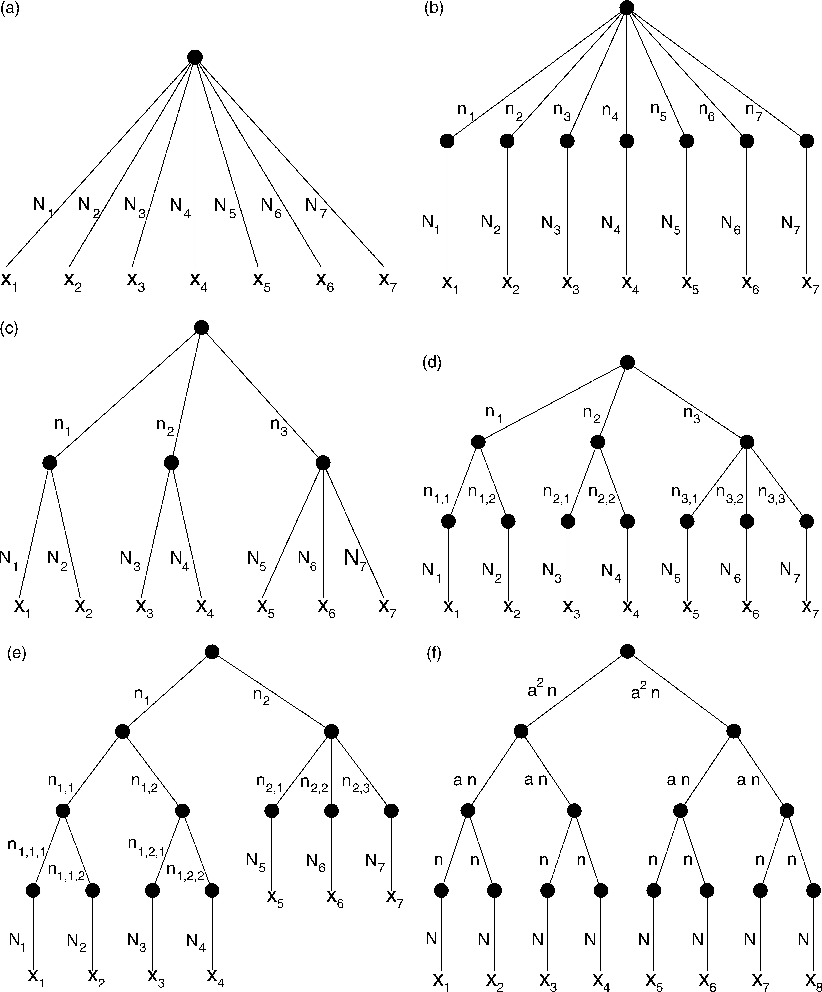
\includegraphics[width=\textwidth]{figures/treeDiagramms}
    \end{subfigure}
    \caption{Unterschiedliche Darstellung von Wellenfunktionen eines siebendimensionalen Systems. Dargestellt sind: (a) Eine Darstellung eines Standardwellenpakets,
      (b) eine MCTDH-Wellenfunktion, (c) eine modenkombinierte MCTDH-Wellenfunktion, [(d)-(f)] eine ML-MCTDH-Wellenfunktion.}\label{fig:tree}

\end{figure}

Anstelle die SPFs aus Gleichung \ref{Eq:mode_comb_wave} in einer primitiven Basen zu entwickeln, k"onnen die SPFs des ersten Layers
durch SPFs eines zweiten Layers dargestellt werden. Die SPFs des ersten Layers werden analog zu einer MCTDH-Wellenfunktion entwickelt.
Diese Entwicklung f"uhrt zu einer ML-MCTDH-Wellenfunktion: 

\begin{equation}
  \begin{gathered}
 \phi^{1;\kappa}_{m} (q^1_{\kappa}, t)=\sum^{n_{\kappa,1}}_{j=1} ... \sum^{n_{\kappa,d_\kappa}}_{j_{d_\kappa}=1} A^{2;\kappa}_{m;j_1,...,j_{d_\kappa}}(t)
 \times \phi^{2;\kappa,1}_{j_1} (q^{2;\kappa}_{1}, t) \cdot ... \cdot
 \phi^{2;\kappa,d_\kappa}_{j_{d_\kappa}} (q^{2;\kappa}_{d_\kappa}, t)
\\
 \phi^{2;\kappa, \lambda}_{m} (q^{2;\kappa}_{\lambda}, t)= \sum^{N_{\alpha}}_{j=1} A^{3;\kappa, \lambda}_{m;j}(t)
 \mathcal{X}^{(\alpha)}_{j}(q^{2;\kappa}_\lambda)
\\
 \left( \text{ mit } \alpha = \lambda + \sum^{\kappa - 1}_{i=1}d_i \right)
 \label{Eq:ml_mctdh_mode_SPF}
\end{gathered}
 \end{equation}

Die Indizes $\kappa$ und $\lambda$ des SPFs des zweiten Layers $ \phi^{2;\kappa, \lambda}_{m}  $  sind durch die Koordinaten und deren
Zugeh"origkeit zu den logischen Koordinate festgelegt.
Die Koeffizienten $A^{2;\kappa}_{m;j_1,...,j_{d_\kappa}}$ definieren weiterhin die Entwicklung der SPFs des ersten Layers.
Allerdings werden anstelle der zeitunbh"angigen primitiven Basis die zeitabh"angigen SPFs des zweiten Layers als Basis verwendet.
Die SPFs werden wiederum in der primitiven Basis entwickelt, wobei diese Entwicklung durch den Koeffzienten  $A^{3;\kappa, \lambda}_{m;j}$
definiert wird.
  \\Die ML-MCTDH Darstellung kann auf eine beliebige Anzahl von Layern erweitert werden.
Dabei kann die Anzahl der Layer f"ur die jeweiligen Koordinaten variieren.
So werden in Abbildung \ref{fig:multi_mctdh_wave} f"ur die Koordinaten $x_1-x_4$ drei Layer und f"ur die Koordinaten $x_5 - x_7$ zwei Layer verwendet.
F"ur die Berechnung gr"o"serer Systeme spielt das modenkombinierte MCTDH eine entscheidende Rolle, allerdings sind im Allgemeinen die Kombinationen
durch den exponentielle Anstieg des Teilchengitters auf die dritte Ordnung begrenzt. \cite{MCTDHreview3}
  \\Im Gegensatz zum modenkombinierte MCTDH skaliert das ML-MCTDH nicht exponentielle.
So skaliert die Gesamtanzahl der $A$-Koeffizienten bei einem $f=2^l$-dimensionalen System mit $l=3$ Layern mit einem Faktor von $(a^4n^{3}/4)f^{3\log_{2}a}$
(f"ur $a>2^{1/3}$). Im untersten Layer werden pro Koordinate $n$ SPFs angenommen, die sich pro Layer um den Faktor $a$ erh"ohen.
Es werden $N$ Basisfunktionen f"ur die primitive Basisdarstellung verwendet.
Da der numerische Aufwand des ML-MCTDHs n"ahrungsweise proportional zu der Anzahl der A-Koeffzienten ist, steigt der numerische Aufwand polynomisch
mit einem maximalen Exponenten von $3\log_{2}a$.\cite{Mreview2}
  \\F"ur die Herleitung der Bewegungsgleichungen im n"achsten Abschnitt werden folgende Notationen eingef"uhrt.
Statt den SPFs k"onnen die MCTDH-Wellenfunktionen durch Einlochfunktionen (SHF) \cite{Mreview2, MCTDHreview3} beschreiben werden:

 \begin{equation}
 \Psi=\sum^{n_{\kappa_1,\kappa_2,...,\kappa_l}}_{i=1} \Psi^{l;\kappa_1,\kappa_2,...,\kappa_l}_{i} \cdot  \phi^{l;\kappa_1,\kappa_2,...,\kappa_l}_{i}
 \label{Eq:MCTDH_SHF}
 \end{equation}

 mit

 \begin{equation}
   \Psi^{l;\kappa_1,\kappa_2,...,\kappa_l}_{i} =  \Braket {\phi^{l;\kappa_1,\kappa_2,...,\kappa_l}_{i} | \Psi}
 \label{Eq:SHF}
 \end{equation}


Die Konfigurationen des l-ten Layers $ \Phi^{\kappa_1,\kappa_2,...,\kappa_{l-1}}_j $ werden durch das Produkt der SPFs definiert:

 \begin{equation}
   \Phi^{\kappa_1,\kappa_2,...,\kappa_{l-1}}_{j_1,...,j_{d_{\kappa_1,..,\kappa_{l-1}}}} = \prod_{\kappa_l}^{d_{\kappa_1,...,\kappa_{l}}}
   \phi^{\kappa_1,\kappa_2,...,\kappa_{l-1},\kappa_l}_{j_{\kappa_l}}.
 \label{Eq:notation}
 \end{equation}

 Durch den Superindexes $ J = (j_1, j_2,...) $ ergibt sich folgende Notation:

 \begin{equation}
   \phi^{\kappa_1,\kappa_2,...,\kappa_{l}}_i = \sum_J A^{l+1;\kappa_1,\kappa_2,...,\kappa_l}_{i;J}
   \cdot \phi^{l+1;\kappa_1,\kappa_2,...,\kappa_{l}}_J
 \label{Eq:superindex}
 \end{equation}

 Des Weiteren wird f"ur die zeitunbh"angigen Basisfunktionen des untersten Layer nicht mehr das Symbol $ \chi_{j_m} $ verwendet.
 Stattdessen werden im folgenden die Basisfunktionen ebenfalls durch die korrespondierenden SPFs $ \phi^{l;\kappa_1,\kappa_2,...,\kappa_{l},m}_{j_m} $
 gekennzeichnet.
